%%%%%%%%%%%%%%%%%%%%%%%%%%%%%%%%%%%%%%%%%%%%%%%%%%%
\begin{frame}
\begin{center}
{\Large ML Course Demo 2 - Customer Churn}
\end{center}

{\tiny (Ref: mlcourse.ai – Open Machine Learning Course \\
 https://www.kaggle.com/kashnitsky/topic-2-visual-data-analysis-in-python) }
\end{frame}

%%%%%%%%%%%%%%%%%%%%%%%%%%%%%%%%%%%%%%%%%%%%%%%%%%%
\begin{frame}[fragile]\frametitle{Import Libraries}
Initialize environment
\begin{lstlisting}
import numpy as np
import pandas as pd

# we don't like warnings
# you can comment the following 2 lines if you'd like to
import warnings
warnings.filterwarnings('ignore')

import matplotlib.pyplot as plt

import seaborn as sns
sns.set()
\end{lstlisting}
\end{frame}

%%%%%%%%%%%%%%%%%%%%%%%%%%%%%%%%%%%%%%%%%%%%%%%%%%%
\begin{frame}[fragile]\frametitle{Load data}
\begin{lstlisting}
df = pd.read_csv('../../data/telecom_churn.csv')
\end{lstlisting}
To get acquainted with our data, let’s look at the first 5 entries using head():
\begin{lstlisting}
df.head()
\end{lstlisting}

\begin{center}
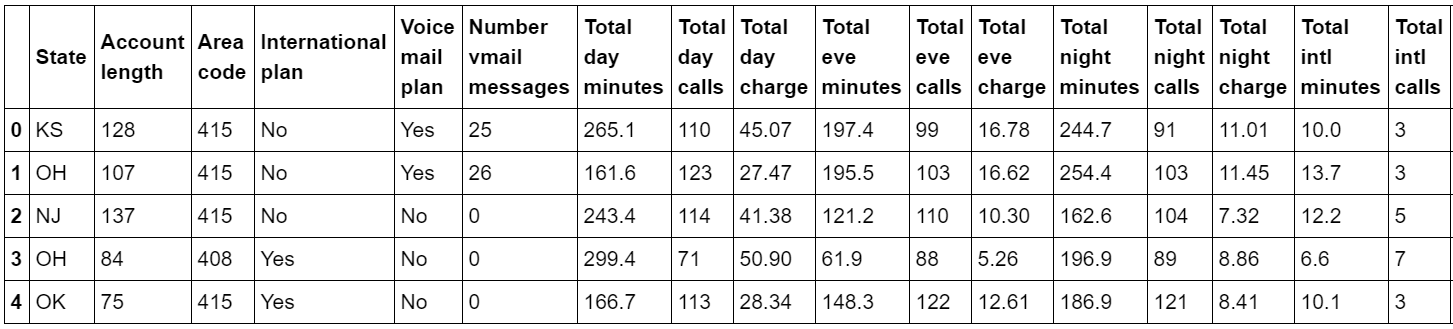
\includegraphics[width=\linewidth,keepaspectratio]{churn27}
\end{center}
\end{frame}


%%%%%%%%%%%%%%%%%%%%%%%%%%%%%%%%%%%%%%%%%%%%%%%%%%%
\begin{frame}[fragile]\frametitle{Describing  the data}
Features
\begin{center}
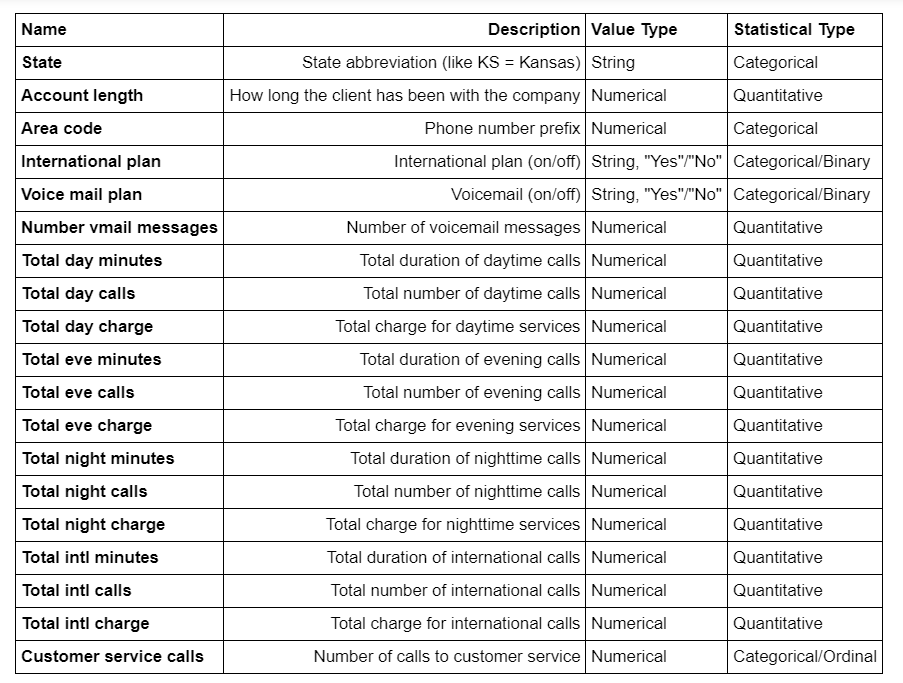
\includegraphics[width=0.65\linewidth,keepaspectratio]{churn28}
\end{center}
The last data column, Churn, is our target variable. It is binary
\end{frame}

%%%%%%%%%%%%%%%%%%%%%%%%%%%%%%%%%%%%%%%%%%%%%%%%%%%%%%%%%%
\begin{frame}[fragile]\frametitle{Univariate visualization}	
\begin{itemize}
\item Univariate analysis looks at one variable at a time. 
\item When we analyze a feature independently, we are usually mostly interested in the distribution of its values and ignore the other variables in the dataset.
\item Quantitative features take on ordered numerical values. Those values can be discrete, like integers, or continuous, like real numbers, and usually express a count or a measurement.
\end{itemize}
\end{frame}

%%%%%%%%%%%%%%%%%%%%%%%%%%%%%%%%%%%%%%%%%%%%%%%%%%%
\begin{frame}[fragile]\frametitle{Histograms}
The easiest way to take a look at the distribution of a numerical variable is to plot its histogram using the DataFrame's method hist()
\begin{lstlisting}
features = ['Total day minutes', 'Total intl calls']
df[features].hist(figsize=(12, 4));
\end{lstlisting}
\begin{center}
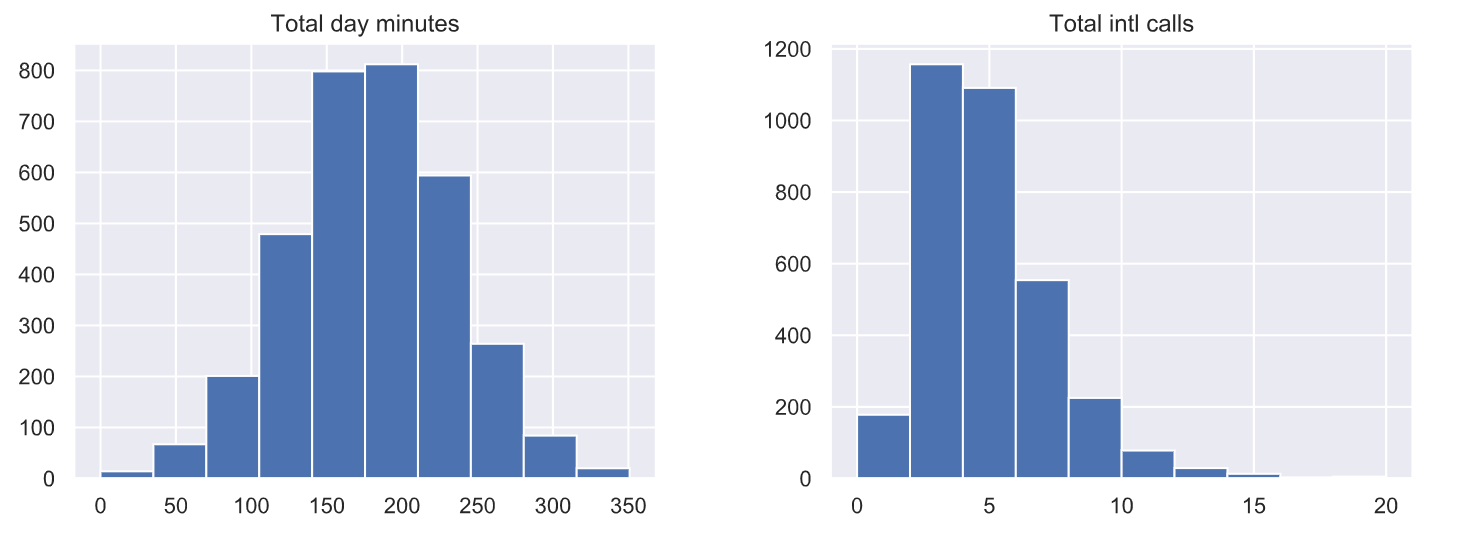
\includegraphics[width=0.8\linewidth,keepaspectratio]{churn29}
\end{center}
We see that the variable Total day minutes is normally distributed, while Total intl calls is prominently skewed right (its tail is longer on the right).
\end{frame}

%%%%%%%%%%%%%%%%%%%%%%%%%%%%%%%%%%%%%%%%%%%%%%%%%%%%%%%%%%
\begin{frame}[fragile]\frametitle{Histograms}
\begin{itemize}
\item A histogram groups values into bins of equal value range. 
\item The shape of the histogram may contain clues about the underlying distribution type: Gaussian, exponential etc. 
\item You can also spot any skewness in its shape when the distribution is nearly regular but has some anomalies. 
\item Knowing the distribution of the feature values becomes important when you use Machine Learning methods that assume a particular type of it, most often Gaussian.
\end{itemize}
\end{frame}


%%%%%%%%%%%%%%%%%%%%%%%%%%%%%%%%%%%%%%%%%%%%%%%%%%%
\begin{frame}[fragile]\frametitle{Density Plots}
Can be considered a smoothed version of the histogram. Their main advantage over the latter is that they do not depend on the size of the bins. Let's create density plots for the same two variables:
\begin{lstlisting}
df[features].plot(kind='density', subplots=True, layout=(1, 2), sharex=False, figsize=(12, 4));
\end{lstlisting}
\begin{center}
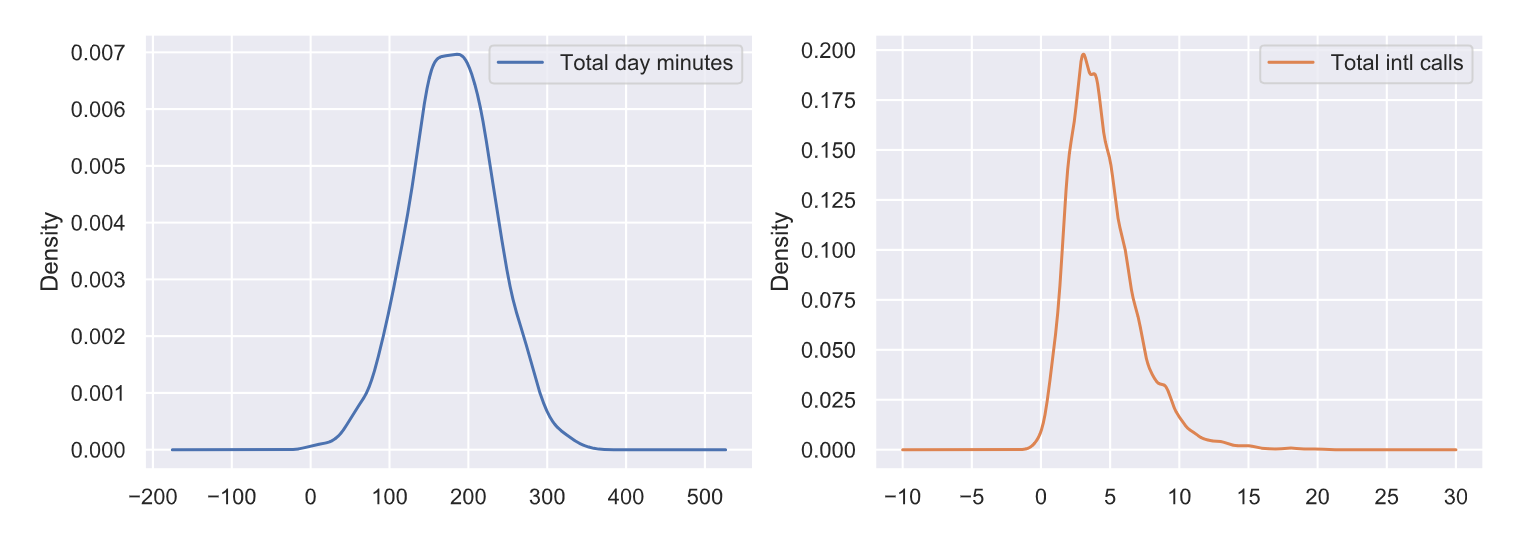
\includegraphics[width=0.8\linewidth,keepaspectratio]{churn30}
\end{center}
\end{frame}


%%%%%%%%%%%%%%%%%%%%%%%%%%%%%%%%%%%%%%%%%%%%%%%%%%%
\begin{frame}[fragile]\frametitle{Density Plots}
 Plot a distribution of observations with seaborn's distplot(). 
 \begin{lstlisting}
sns.distplot(df['Total intl calls']);
\end{lstlisting}
\begin{center}
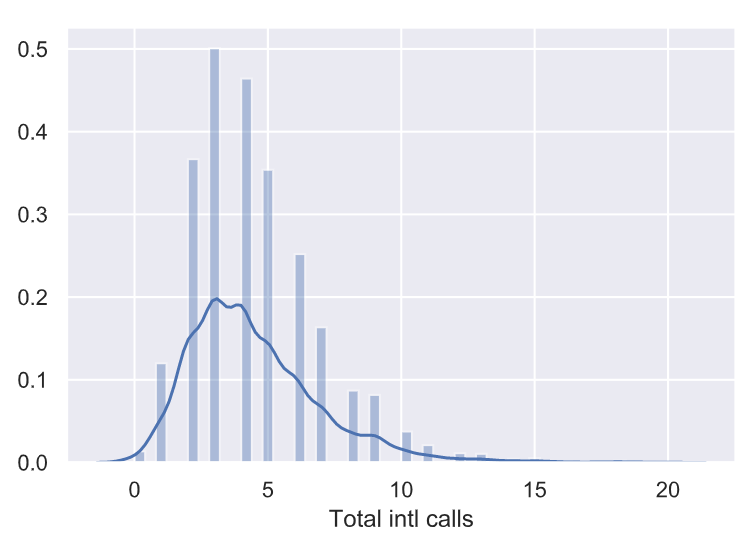
\includegraphics[width=0.5\linewidth,keepaspectratio]{churn31}
\end{center}
The height of the histogram bars here is normed and shows the density rather than the number of examples in each bin.
\end{frame}


%%%%%%%%%%%%%%%%%%%%%%%%%%%%%%%%%%%%%%%%%%%%%%%%%%%
\begin{frame}[fragile]\frametitle{Box Plots}
 Plot a distribution of observations with seaborn's distplot(). 
 \begin{lstlisting}
_, ax = plt.subplots(figsize=(3, 4))
sns.boxplot(data=df['Total intl calls'], ax=ax);
\end{lstlisting}
\begin{center}
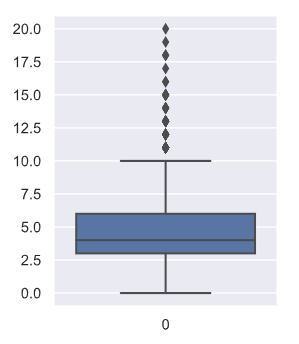
\includegraphics[width=0.45\linewidth,keepaspectratio]{churn32}
\end{center}

\end{frame}

%%%%%%%%%%%%%%%%%%%%%%%%%%%%%%%%%%%%%%%%%%%%%%%%%%%
\begin{frame}[fragile]\frametitle{Box Plots}
\begin{itemize}
\item Length is determined by the  25th(Q1)  and  75th(Q3)  percentiles. 
\item Line inside the box marks the median ( 50\% ) of the distribution.
\item Whiskers represent  the interval $(\text{Q1} - 1.5 \cdot \text{IQR}, \text{Q3} + 1.5 \cdot \text{IQR})$ , where  $\text{IQR} = \text{Q3} - \text{Q1}$
\item Outliers that fall out of the range bounded by the whiskers are plotted individually as black points along the central axis.
\item We can see that a large number of international calls is quite rare in our data.
\end{itemize}

\end{frame}

%%%%%%%%%%%%%%%%%%%%%%%%%%%%%%%%%%%%%%%%%%%%%%%%%%%
\begin{frame}[fragile]\frametitle{Bar Plots}
The bar plot is a graphical representation of the frequency table.
 \begin{lstlisting}
_, axes = plt.subplots(nrows=1, ncols=2, figsize=(12, 4))

sns.countplot(x='Churn', data=df, ax=axes[0]);
sns.countplot(x='Customer service calls', data=df, ax=axes[1]);
\end{lstlisting}
\begin{center}
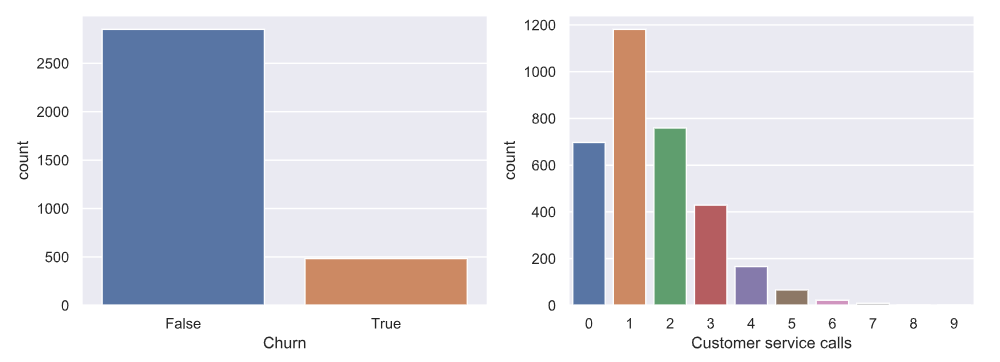
\includegraphics[width=0.6\linewidth,keepaspectratio]{churn33}
\end{center}
The left chart above vividly illustrates the imbalance in our target variable. The bar plot for Customer service calls on the right gives a hint that the majority of customers resolve their problems in maximum 2–3 calls.
\end{frame}

%%%%%%%%%%%%%%%%%%%%%%%%%%%%%%%%%%%%%%%%%%%%%%%%%%%
\begin{frame}[fragile]\frametitle{Bar Plots}
While the histograms, discussed above, and bar plots may look similar, there are several differences between them:
\begin{itemize}
\item Histograms are best suited for looking at the distribution of numerical variables while bar plots are used for categorical features.
\item The values on the X-axis in the histogram are numerical; a bar plot can have any type of values on the X-axis: numbers, strings, booleans.
\item The histogram's X-axis is a Cartesian coordinate axis along which values cannot be changed; the ordering of the bars is not predefined. Still, it is useful to note that the bars are often sorted by height, that is, the frequency of the values. Also, when we consider ordinal variables (like Customer service calls in our data), the bars are usually ordered by variable value.
\end{itemize}
\end{frame}

%%%%%%%%%%%%%%%%%%%%%%%%%%%%%%%%%%%%%%%%%%%%%%%%%%%
\begin{frame}[fragile]\frametitle{Multivariate visualization}
\begin{itemize}
\item Multivariate plots allow us to see relationships between two and more different variables, all in one figure. 
\item Depends on type of variables
\item Quantitative–Quantitative: Correlation matrix, Scatter plot, Scatterplot matrix
\item  Quantitative–Categorical
\item Categorical–Categorical
\end{itemize}

\end{frame}

%%%%%%%%%%%%%%%%%%%%%%%%%%%%%%%%%%%%%%%%%%%%%%%%%%%
\begin{frame}[fragile]\frametitle{Correlation matrix}
\begin{itemize}
\item First, we will use the method corr() on a DataFrame that calculates the correlation between each pair of features. 
\item Then, we pass the resulting correlation matrix to heatmap() from seaborn, which renders a color-coded matrix for the provided values
\end{itemize}
 \begin{lstlisting}
# Drop non-numerical variables
numerical = list(set(df.columns) - 
                 set(['State', 'International plan', 'Voice mail plan', 
                      'Area code', 'Churn', 'Customer service calls']))

# Calculate and plot
corr_matrix = df[numerical].corr()
sns.heatmap(corr_matrix);
\end{lstlisting}
\end{frame}

%%%%%%%%%%%%%%%%%%%%%%%%%%%%%%%%%%%%%%%%%%%%%%%%%%%
\begin{frame}[fragile]\frametitle{Correlation matrix}
\begin{center}
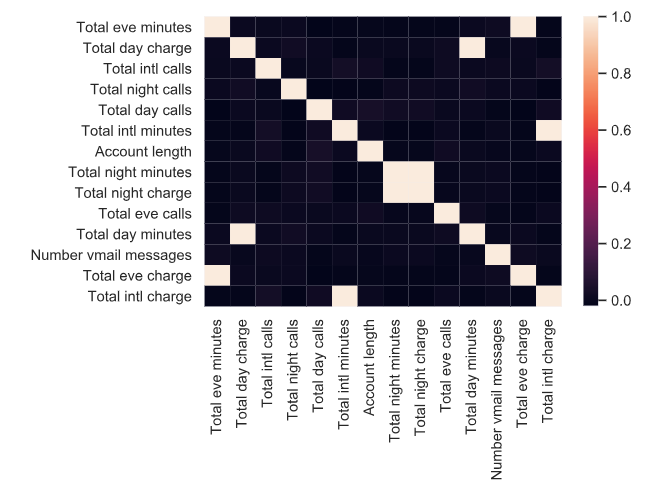
\includegraphics[width=0.5\linewidth,keepaspectratio]{churn34}
\end{center}
 4 variables such as Total day charge that have been calculated directly from the number of minutes spent on phone calls (Total day minutes). These are called dependent variables and can therefore be left out since they do not contribute any additional information.
 \end{frame}

%%%%%%%%%%%%%%%%%%%%%%%%%%%%%%%%%%%%%%%%%%%%%%%%%%%
\begin{frame}[fragile]\frametitle{Scatter Plots}
The scatter plot displays values of two numerical variables as Cartesian coordinates in 2D space. 3D are also possible.
 \begin{lstlisting}
plt.scatter(df['Total day minutes'], df['Total night minutes']);
\end{lstlisting}
\begin{center}
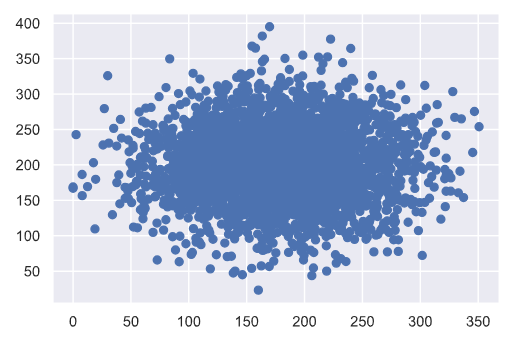
\includegraphics[width=0.45\linewidth,keepaspectratio]{churn35}
\end{center}
We get an uninteresting picture of two normally distributed variables. Also, it seems that these features are uncorrelated because the ellpise-like shape is aligned with the axes.
\end{frame}


%%%%%%%%%%%%%%%%%%%%%%%%%%%%%%%%%%%%%%%%%%%%%%%%%%%
\begin{frame}[fragile]\frametitle{Scatter Plots}
A slightly fancier option to create a scatter plot with the seaborn library:
 \begin{lstlisting}
sns.jointplot(x='Total day minutes', y='Total night minutes', 
              data=df, kind='scatter');
\end{lstlisting}
\begin{center}
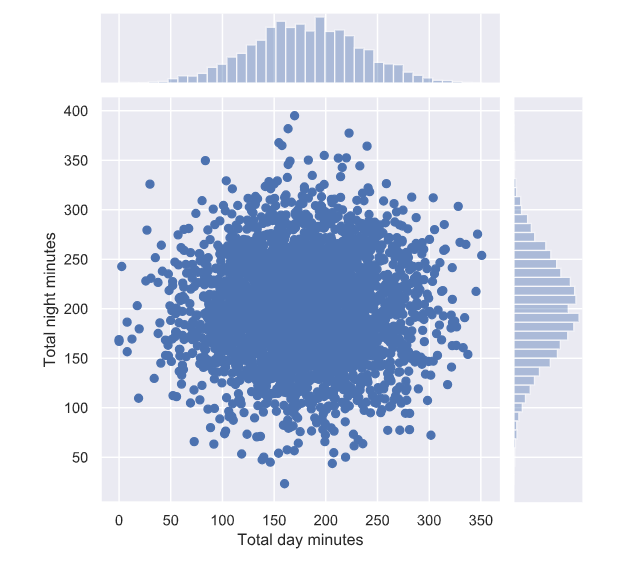
\includegraphics[width=0.45\linewidth,keepaspectratio]{churn36}
\end{center}
\end{frame}


%%%%%%%%%%%%%%%%%%%%%%%%%%%%%%%%%%%%%%%%%%%%%%%%%%%
\begin{frame}[fragile]\frametitle{Scatter Plots}
Using the same function, we can also get a smoothed version of our bivariate distribution:
 \begin{lstlisting}
sns.jointplot('Total day minutes', 'Total night minutes', data=df,
              kind="kde", color="g");
\end{lstlisting}
\begin{center}
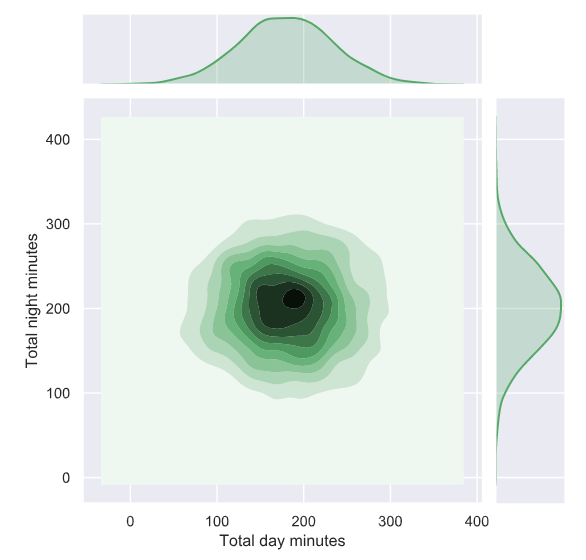
\includegraphics[width=0.45\linewidth,keepaspectratio]{churn37}
\end{center}
\end{frame}

%%%%%%%%%%%%%%%%%%%%%%%%%%%%%%%%%%%%%%%%%%%%%%%%%%%
\begin{frame}[fragile]\frametitle{Scatter Plots Matrix}
Its diagonal contains the distributions of the corresponding variables, and the scatter plots for each pair of variables fill the rest of the matrix.
 \begin{lstlisting}
sns.pairplot(df[numerical]);
\end{lstlisting}
\begin{center}
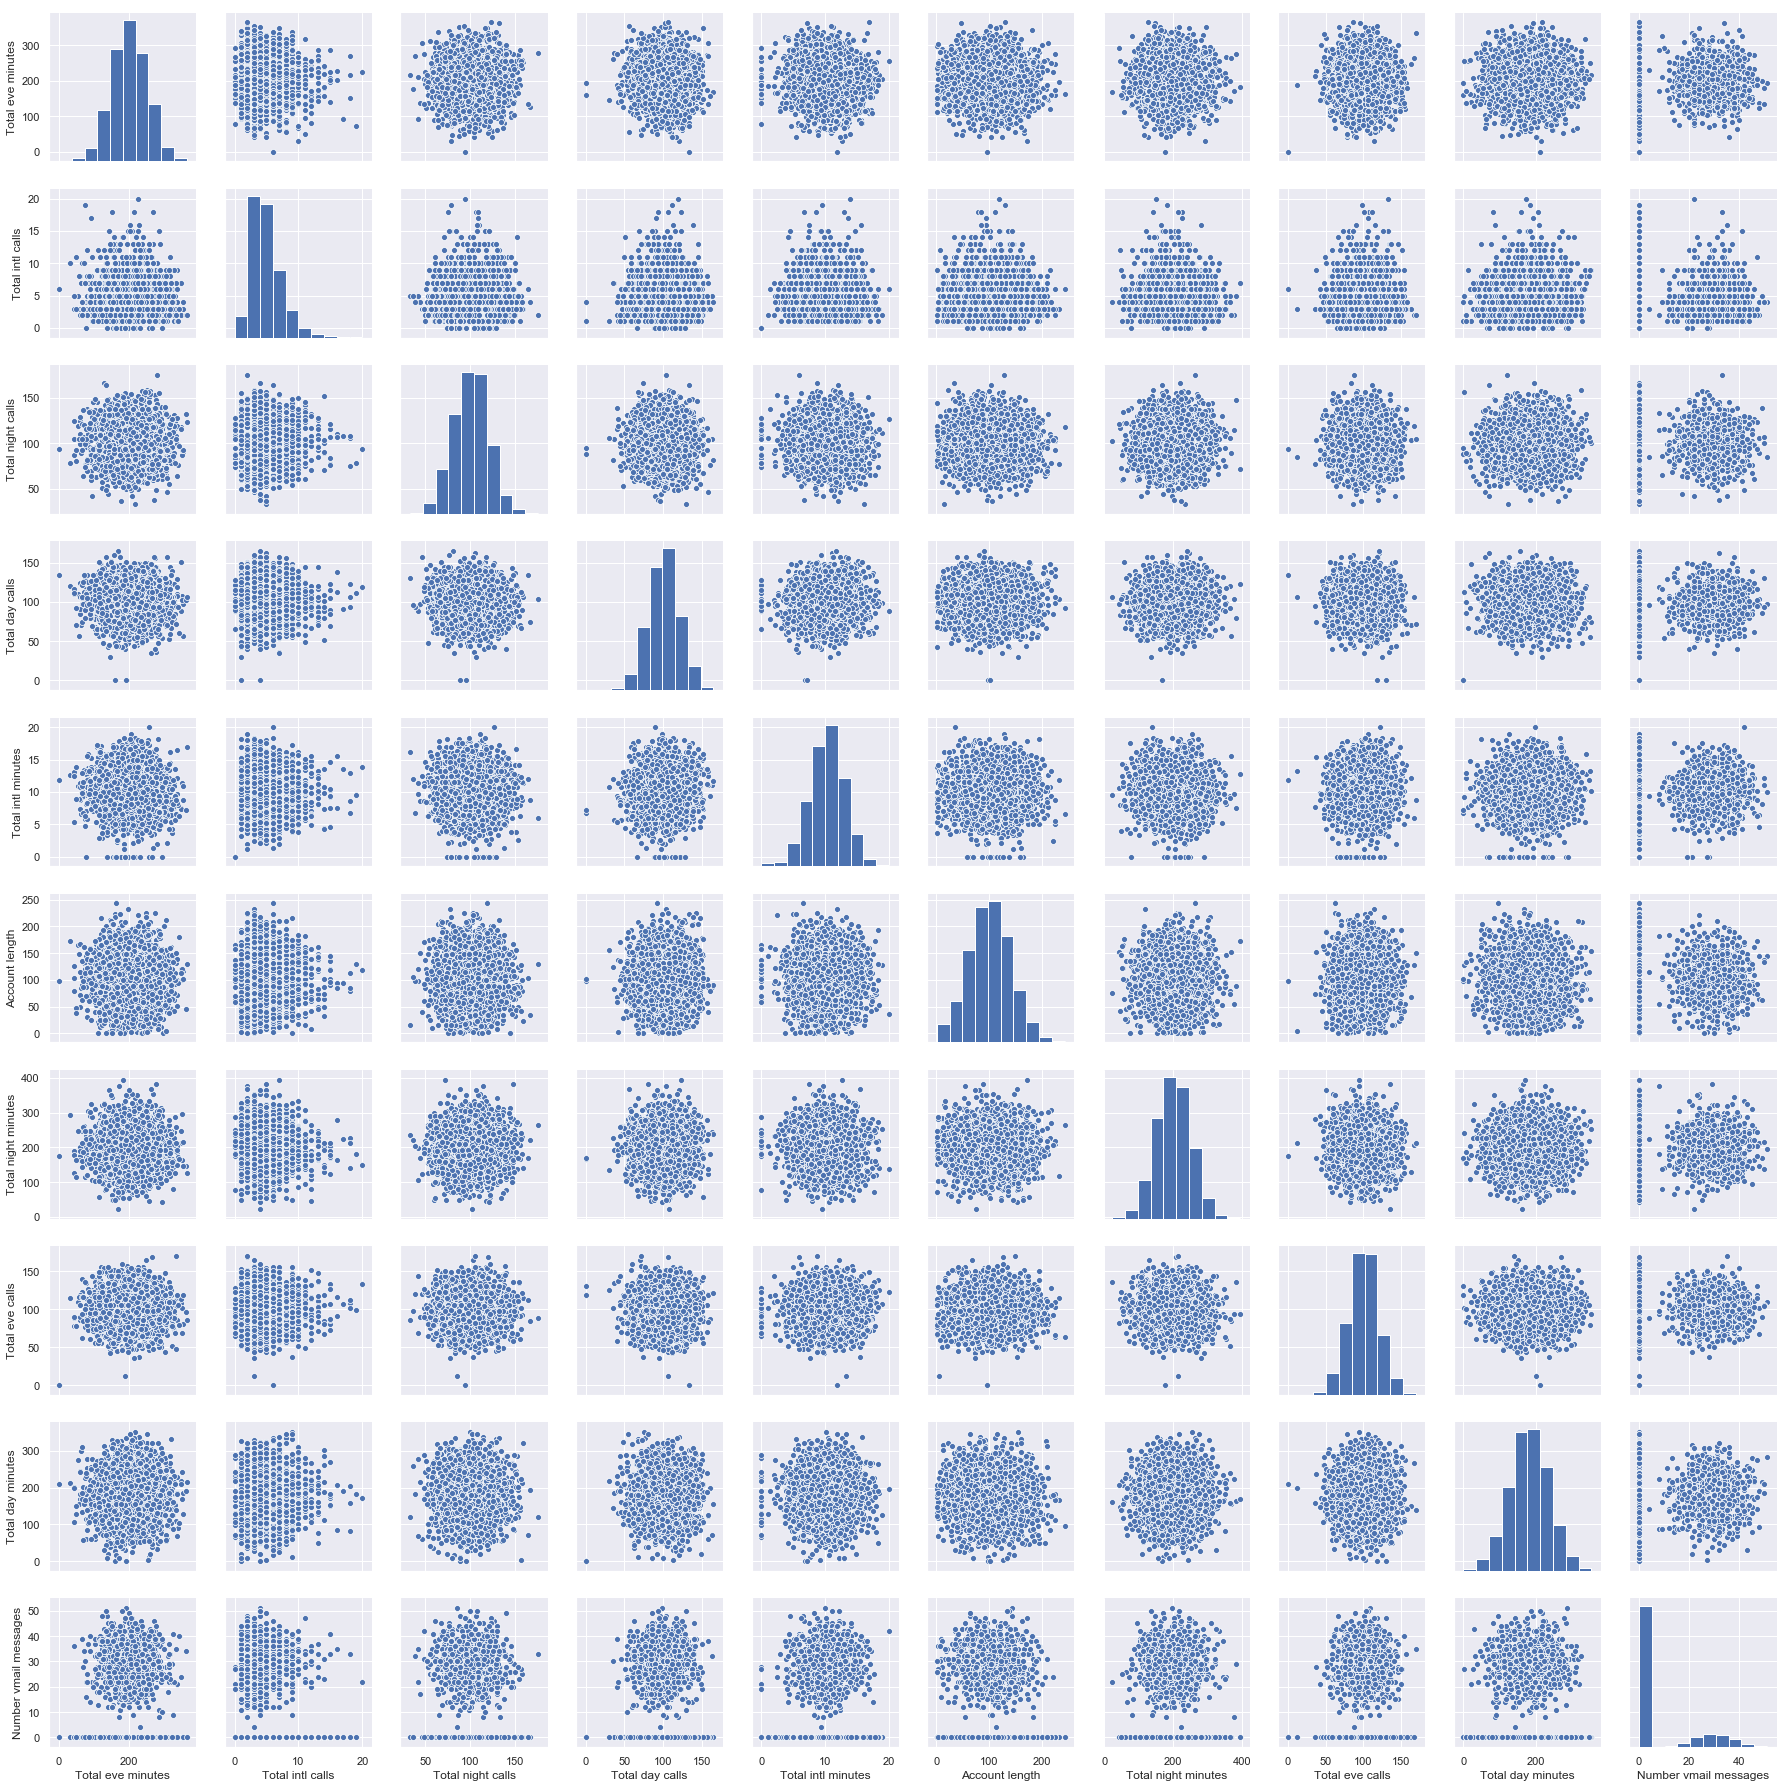
\includegraphics[width=0.45\linewidth,keepaspectratio]{churn38}
\end{center}
\end{frame}

%%%%%%%%%%%%%%%%%%%%%%%%%%%%%%%%%%%%%%%%%%%%%%%%%%%
\begin{frame}[fragile]\frametitle{Quantitative–Categorical}
\begin{itemize}
\item  Let's see how the input variables are related to the target variable Churn
\item Scatter plot points can be color or size coded so that the values of a third categorical variable are also presented in the same figure. 
\item We can achieve this with the scatter() function seen above, but, let's try a new function called lmplot() and use the parameter hue to indicate our categorical feature of interest
\end{itemize}
 \begin{lstlisting}
sns.lmplot('Total day minutes', 'Total night minutes', data=df, hue='Churn', fit_reg=False);
\end{lstlisting}
\end{frame}

%%%%%%%%%%%%%%%%%%%%%%%%%%%%%%%%%%%%%%%%%%%%%%%%%%%
\begin{frame}[fragile]\frametitle{Scatter Plots}
\begin{center}
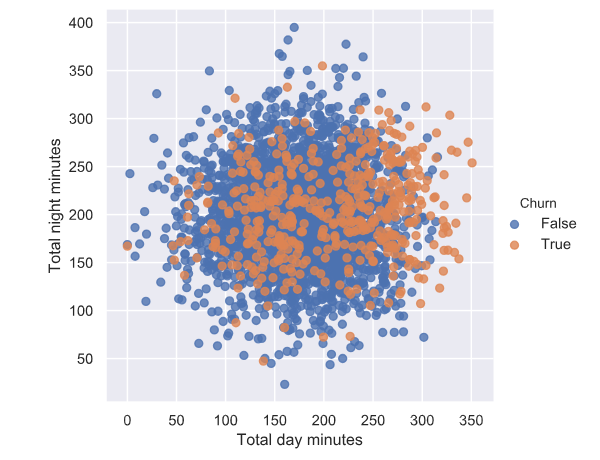
\includegraphics[width=0.45\linewidth,keepaspectratio]{churn39}
\end{center}
It seems that our small proportion of disloyal customers lean towards the top-right corner; that is, such customers tend to spend more time on the phone during both day and night. But this is not absolutely clear, and we won't make any definitive conclusions from this chart.
\end{frame}

%%%%%%%%%%%%%%%%%%%%%%%%%%%%%%%%%%%%%%%%%%%%%%%%%%%
\begin{frame}[fragile]\frametitle{Box Plots}
 Let's create box plots to visualize the distribution statistics of the numerical variables in two disjoint groups: the loyal customers (Churn=False) and those who left (Churn=True).
 \begin{lstlisting}
# Sometimes you can analyze an ordinal variable just as numerical one
numerical.append('Customer service calls')

fig, axes = plt.subplots(nrows=3, ncols=4, figsize=(10, 7))
for idx, feat in enumerate(numerical):
    ax = axes[int(idx / 4), idx % 4]
    sns.boxplot(x='Churn', y=feat, data=df, ax=ax)
    ax.set_xlabel('')
    ax.set_ylabel(feat)
fig.tight_layout();
\end{lstlisting}
\end{frame}

%%%%%%%%%%%%%%%%%%%%%%%%%%%%%%%%%%%%%%%%%%%%%%%%%%%
\begin{frame}[fragile]\frametitle{Box Plots}
\begin{center}
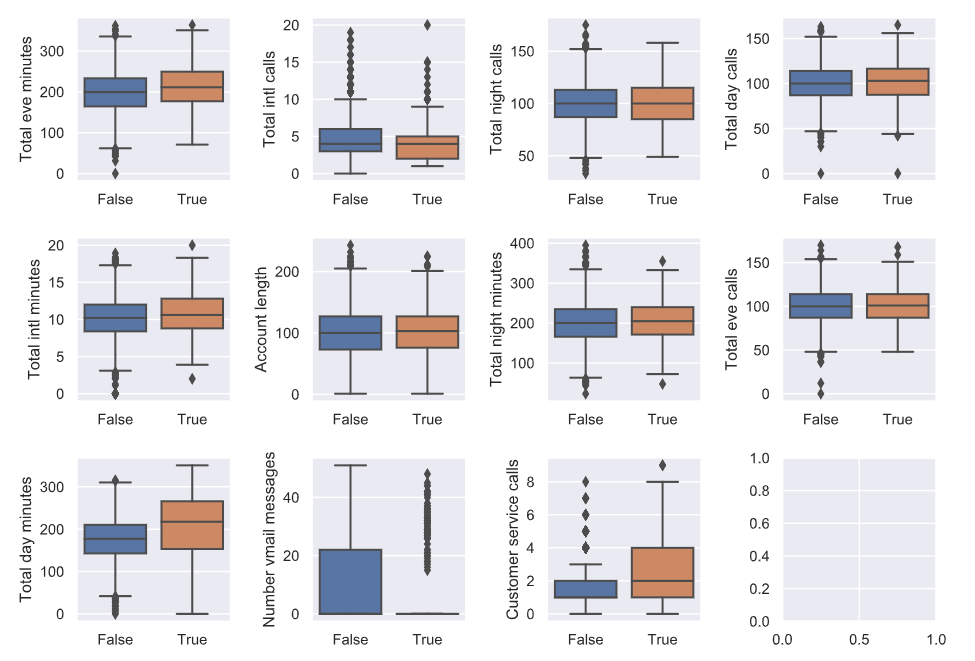
\includegraphics[width=0.6\linewidth,keepaspectratio]{churn40}
\end{center}
The greatest discrepancy in distribution between the two groups is for three variables: Total day minutes, Customer service calls, and Number vmail messages. 
\end{frame}

%%%%%%%%%%%%%%%%%%%%%%%%%%%%%%%%%%%%%%%%%%%%%%%%%%%
\begin{frame}[fragile]\frametitle{Box Plots}
Let's look at the distribution of day minutes spoken for the loyal and disloyal customers separately. We will create box and violin plots for Total day minutes grouped by the target variable.
 \begin{lstlisting}
_, axes = plt.subplots(1, 2, sharey=True, figsize=(10, 4))

sns.boxplot(x='Churn', y='Total day minutes', data=df, ax=axes[0]);
sns.violinplot(x='Churn', y='Total day minutes', data=df, ax=axes[1]);
\end{lstlisting}
\begin{center}
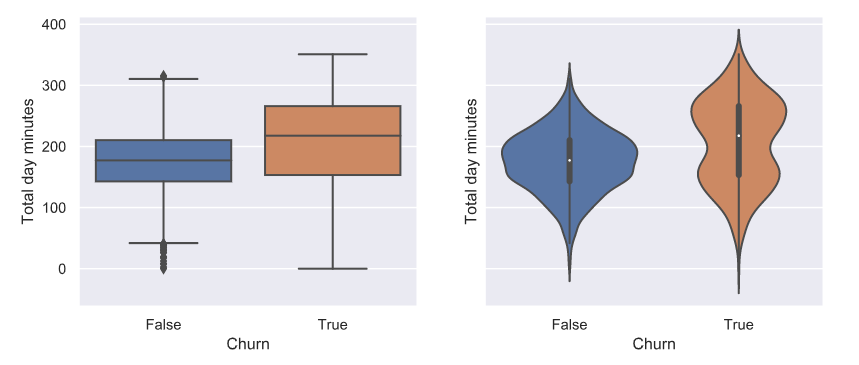
\includegraphics[width=0.45\linewidth,keepaspectratio]{churn41}
\end{center}
\end{frame}

%%%%%%%%%%%%%%%%%%%%%%%%%%%%%%%%%%%%%%%%%%%%%%%%%%%
\begin{frame}[fragile]\frametitle{An interesting observation}
\begin{itemize}
\item On average, customers that discontinue their contracts are more active users of communication services. 
\item Perhaps they are unhappy with the tariffs, so a possible measure to prevent churn could be a reduction in call rates. 
\item The company will need to undertake additional economic analysis to find out whether such measures would be beneficial.
\end{itemize}
\end{frame}

%%%%%%%%%%%%%%%%%%%%%%%%%%%%%%%%%%%%%%%%%%%%%%%%%%%
\begin{frame}[fragile]\frametitle{Box Plots}
When we want to analyze a quantitative variable in two categorical dimensions at once, there is a suitable function for this in the seaborn library called factorplot(). For example, let's visualize the interaction between Total day minutes and two categorical variables in the same plot:
 \begin{lstlisting}
sns.factorplot(x='Churn', y='Total day minutes', col='Customer service calls',
               data=df[df['Customer service calls'] < 8], kind="box",
               col_wrap=4, size=3, aspect=.8);
\end{lstlisting}
\end{frame}

%%%%%%%%%%%%%%%%%%%%%%%%%%%%%%%%%%%%%%%%%%%%%%%%%%%
\begin{frame}[fragile]\frametitle{Box Plots}
\begin{center}
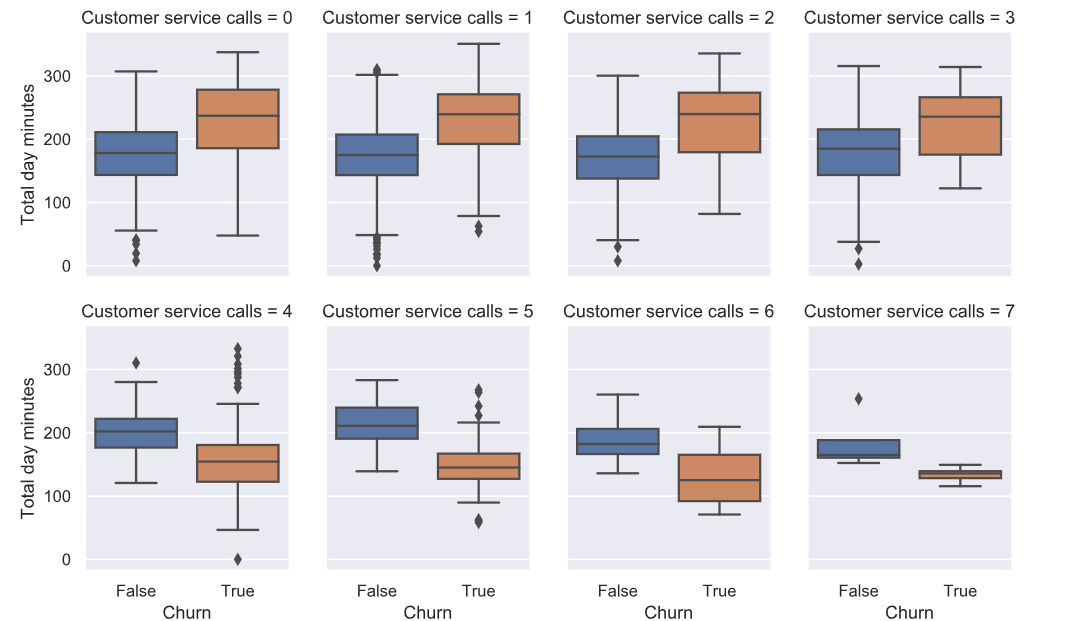
\includegraphics[width=0.45\linewidth,keepaspectratio]{churn42}
\end{center}
From this, we could conclude that, starting with 4 calls, Total day minutes may no longer be the main factor for customer churn. Perhaps, in addition to our previous guess about the tariffs, there are customers that are dissatisfied with the service due to other problems, which might lead to fewer number of day minutes spent on calls.
\end{frame}

%%%%%%%%%%%%%%%%%%%%%%%%%%%%%%%%%%%%%%%%%%%%%%%%%%%
\begin{frame}[fragile]\frametitle{Categorical–Categorical}
Let's look at the distribution of the number of calls to the customer service, again using a count plot. This time, let's also pass the parameter hue=Churn that adds a categorical dimension to the plot:
 \begin{lstlisting}
sns.countplot(x='Customer service calls', hue='Churn', data=df);
\end{lstlisting}
\end{frame}

%%%%%%%%%%%%%%%%%%%%%%%%%%%%%%%%%%%%%%%%%%%%%%%%%%%
\begin{frame}[fragile]\frametitle{Categorical–Categorical}
\begin{center}
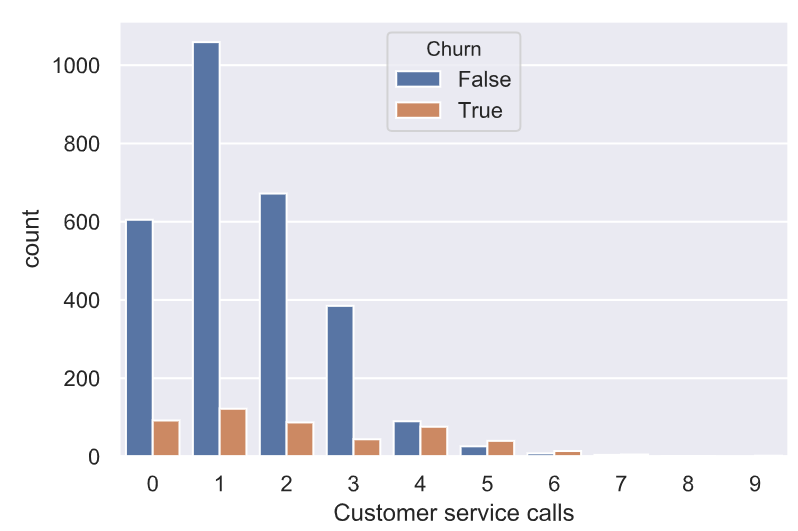
\includegraphics[width=0.6\linewidth,keepaspectratio]{churn43}
\end{center}
An observation: the churn rate increases significantly after 4 or more calls to the customer service.
\end{frame}



%%%%%%%%%%%%%%%%%%%%%%%%%%%%%%%%%%%%%%%%%%%%%%%%%%%
\begin{frame}[fragile]\frametitle{Categorical–Categorical}
Now, let's look at the relationship between Churn and the binary features, International plan and Voice mail plan.
 \begin{lstlisting}
_, axes = plt.subplots(1, 2, sharey=True, figsize=(10, 4))

sns.countplot(x='International plan', hue='Churn', data=df, ax=axes[0]);
sns.countplot(x='Voice mail plan', hue='Churn', data=df, ax=axes[1]);
\end{lstlisting}
\end{frame}

%%%%%%%%%%%%%%%%%%%%%%%%%%%%%%%%%%%%%%%%%%%%%%%%%%%
\begin{frame}[fragile]\frametitle{Categorical–Categorical}
\begin{center}
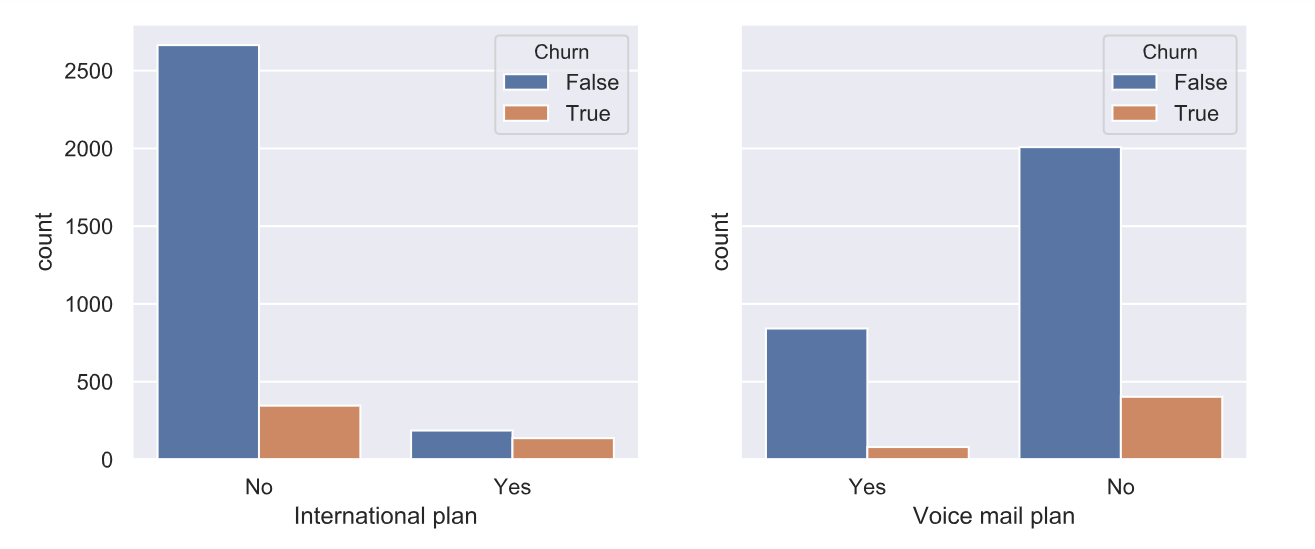
\includegraphics[width=0.6\linewidth,keepaspectratio]{churn44}
\end{center}
An observation: when International Plan is enabled, the churn rate is much higher; the usage of the international plan by the customer is a strong feature. We do not observe the same effect with Voice mail plan.
\end{frame}